\documentclass{article}

\usepackage[french, english]{babel}
\usepackage[T1]{fontenc}
\usepackage[utf8]{inputenc}
\usepackage[ a4paper, hmargin={1cm, 1cm}, vmargin={2cm, 2cm}]{geometry}
\usepackage{hyperref}
\usepackage{biblatex}
\usepackage{url}
\usepackage{multicol}
\usepackage{graphicx}

\title{\textbf{Reports on various readings}}
\author{\textit{Abel HENRY-LAPASSAT}}
\setlength{\parskip}{0.5em}

\begin{document}
\maketitle
\section*{\underline{Quick Explanation}}
    \paragraph{ \textnormal{This document is meant to contains all the readings and understandings I'll do during my HCI Internship.
        So basically, I'll be putting in here some articles and what I understood and thought about their topics and conclusions/results.
        The second goal of this is to start using Latex to write documents, so don't worry if you find some weird stuff, it either is the
        result of shameful mistakes of mine or simply dumb experiences I've done and didn't erase. } }

\section*{\underline{Articles Summary}}
    \begin{itemize}
        \item \href{https://hal.science/hal-04010673/document}{Evaluating the Extension of Wall Displays with AR for Collaborative Work} \dotfill \pageref{sec:james2023}
        \item \href{https://hal.science/hal-01437091/document}{CoReach: Cooperative Gestures for Data Manipulation on Wall-Sized Displays} \dotfill \pageref{sec:liu2017}
        \item \href{https://hal.science/file/index/docid/957269/filename/chi14-classify-hal-v1.pdf}{Effects of Display Size And Navigation Type on a Classification Task} \dotfill \pageref{sec:liu2014}
        \item \href{https://inria.hal.science/hal-01275535/file/CHI16-sharedinteraction-halv1.pdf}{Shared Interaction on a Wall-Sized Display in a Data Manipulation Task} \dotfill \pageref{sec:liu2016}
    \end{itemize}

\section*{\underline{Article Reports}}

    \label{sec:james2023}
    \subsection{Evaluating the Extension of Wall Displays with AR for Collaborative Work}
    \subparagraph{by : R.James, A.Bezerianos, O.Chapuis}
    \cite{james2023evaluating}
    \paragraph{ \textit{Quick Summary :} 
                \newline
                \indent \indent \textnormal{In this article, the researchers are trying to offer a proper way to extend the unused space
                of a LHRD room. In order to do that, and after reading related work about the already existings uses of AR with other physical Displays
                they came with an idea and prototype of wall-extension using AR. }
                \indent \indent \textnormal{So as almost every good paper, this one contains a part about the user studies and results, which I won't 
                comment as much as the rest for obvious reasons, even tho I'll comment it quickly because it's a part of the research.} }
    
    \paragraph{ \textit{The Idea \& Experiment:} 
                \newline
                \indent \indent \textnormal{This article is about extending a LHRD in order to upgrade the vizualisation and manipulation of datas by two
                users collaboratively. For that the idea was to create a Virtual environment around the WallDisplay using AR technology. And uprising the following questions :
                \newline \indent "Is the extension useful ?" 
                \newline \indent "How the AR space is used ?"
                \newline \indent "Does the addition of AR affect collaboration strategy ?"
                \newline \indent "What's the cost of adding AR ?"}
                \indent \indent \textnormal{In order to answer these questions and produce clear and useable datas, an experiment was thought and made up by the searchers. 
                The Idea of this experiment was to show both participant a bunch of dixit images with specific tasks to execute with em, in these tasks were a classification 
                one using storytelling and loose collaboration (aim is to enforce coupled-collaboration), and a much simpler classification task (simply regroup cards by colors 
                for example) which would involve participant self decisions and selections. Moreover, tasks have been done with various contexts, some realized only with the wall,
                and others with both Wall+AR, in order to compare properly the logs and collected datas.}}

    \paragraph{ \textit{Results \& Review :} 
                \newline
                \indent \indent \textnormal{After the experiment, it apperared that the manipulations between the case with/without addition of AR were signlificantly different
                not especially from a performance sight at first, but on the used strategies. But even tho theses strategies were a kind of linked when it was about classification. 
                In fact group were cutting the wall onto 3 different spaces or they created 2 additional spaces to obtain 3 separated ones. The main changes were on the tasks repartition,
                it appears that with the addition of AR, tasks were divided more significantly between participants. And it also became clear that adding AR was useful to overcome the lack 
                of space on the wall.}
                \newline
                \indent \indent \textnormal{And then for the Storytelling task, the collaboration between couples was (as excpected) way closer, and globally groups were working
                in pair thoughts (selecting all 10 cards together). The addition of AR helped the groups to create their story separatedly from the rest of the cards, but in contrast with 
                the classification tasks, the strategy weren't modified at all by this extension of the wall.}
                \newline
                \indent \indent \textnormal{An interesting log that appears in this research is the amount and quality of interactions measured, it shows that globally, the addition of a 
                personnal space was appreciated by most of the groups, and furthermore, the addition of extension wasn't increasing that much the amount of interactions, perhaps it simply made
                their quality better ?}
                \newline
                \indent \indent \textnormal{About all the other logs, we can mainly see differences between Wall \& Wall+AR, participants were moving much more when virtual surface were allowed,
                and card would be manipulated a bit more for the classification in Wall+AR, and the task time was decreased by the addition of virtual stuff, even tho the distance between participant
                had increase, not significantly enough to status on the non-quality of a Wall+AR collaboration tho.} }

    \paragraph{ \textit{Questionnaries :}
                \newline
                \indent \indent \textnormal{Shall I talk about these ??}}
    
    \paragraph{ \textit{Discussion :} 
                \newline
                \indent \indent \textnormal{It was globally observed that beside excpectations of a "secondary use" for the virtual surfaces, they were used as a main component whenever they were 
                allowed. Another main feedback was that the wall alone restricted the possibilities by the lack of space to use. The question subasked by this is the following, are these observations 
                the result of the AR technology, or people would feel the same with physical displays ? Well in fact with physical displays it wouldn't be possible to manipulate objects with such fluidity
                . And as the previous works were all focused on AR, we don't know (at least it's not proved yet) if there would be a true lack of freedom with physical surfaces. Another thing that is interestingly
                mentionned is that the resolution of LHRD are way superior to what we have in AR headsets yet, so there's a question "What if all the surfaces were displayed with AR ?" .}
                \newline
                \indent \indent \textnormal{Also the AR space, that was meant to fulfill all the empty space of a single wall, was mainly created on both sides of the wall, which was one of the principal purpose of this research.
                Overall, the different surfaces were seen as "territories", which could be related to the personnal aspect of such AR surfaces. These reflected a feeling of ownership throughout the experiment when using the surface
                that was on a specific participant side.}
                \newline
                \indent \indent \textnormal{The addition of AR has engendered changes only for the classification task, as for the story nothing really changed, in fact it has "normalized" the different strategies. In fact with only 
                the Wall, there were most different strategies than with the Wall+AR, were all strategies were much more similar. The conclusion on this point is that a restricted area might favorize a tighter collaboration \& coordination.}
                \newline
                \indent \indent \textnormal{Furthermore there really is a trade-off when adding AR to a LHRD, because even tho the Wall+AR interface is more efficient, it demands more mental and physical efforts. But for this point, I personnaly
                don't think this is a real problem, in fact on one-hand we don't want people to do to much efforts but are these effort enoughly significant to consider them as a problem ? Another more defendable point for me 
                would be that in the measured interactions, there are fewer actions when it cames to Wall+AR. But overcoming that, the Wall+AR setup has been enjoyed much more than the single Wall, is that because people prefer to work all by their
                own ? Well I don't know but for me there are more advantages than problems caused to the addition of AR.} }

    \paragraph{ \textit{Conclusion :}
                \newline 
                \indent \indent \textnormal{Globally, these results are a bit complicated to generalize to other configurations, in fact the one used throughout the research appeared to be 
                really good one, and the conclusion of this paper is that the benefits \& drawbacks of such combination aren't clear at all. Because it highlights that this addition is useful for sure, as when AR was added, the virtual 
                surfaces were even more used than the Wall itself. Main questions are about what it would lead to in other extended practices.}
                \newline 
                \indent \indent \textnormal{But, this researxh mainly demonstrates that this addition is feasible and beneficial over any drawbacks it engenders.}}
    \newpage 

    \label{sec:liu2017}
    \subsection*{Effects of Display Size and Navigation Type on a Classification Task}
    \subparagraph{by : C.Liu, O.Chapuis, M.Beaudouin-Lafon, E.Lecolinet, W.Mackay}
    \cite{liu2017CoReach}
    \paragraph{ \textit{Quick Summary :} 
                \newline
                \indent \indent \textnormal{This research papers offers a set of Gestures that would allow users of LHRD to interact more
                easily with the contents they wanna manipulate. As the general multi-touch displays are using pretty common ones, these doesn't 
                scale well with a wall-sized display.}
                \newline
                \indent \indent \textnormal{In this paper, the main worked points are about co-located collaborative navigations, which involves
                more complex dynamics when you're aware of problems like "gorilla-arm" or simply the loss of precision for precise manipulation gestures. 
                Also the \textit{CoReach} set of gestures had to be thought taking care of multiples human factors, such as collaborative strtategies, 
                or even physical constraints.}
                \newline
                \indent \indent \textnormal{Especially, this research focuses on Collaborative interactions, as most (if not every) of the previous works
                did focus on addressing precision and fatigue problems for single-users. To recap, \textit{CoReach} focuses on Large Scale Interaction \& 
                MultiUser Cooperative Actions.} }
    
    \paragraph{ \textit{Motivations :} 
                \newline
                \indent \indent \textnormal{With the rise of dat-driven decision making, scenarios where people face communication barriers due to domain-specific 
                terms are becomming common place. And as a solution to this problem comes the large interactive spaces, and especially as we're talking about datas 
                visualization and manipulation, LHRDs !} }

    \paragraph{\textit{Gestures:} \newline}
    \indent \indent Obviously, what would be a set of gestures without any gestures ? So here is a scheme showing and explaning the three different
    implemented gestures for the \textit{CoReach} prototype :
    
                
    \begin{figure}[h]
        \centering
        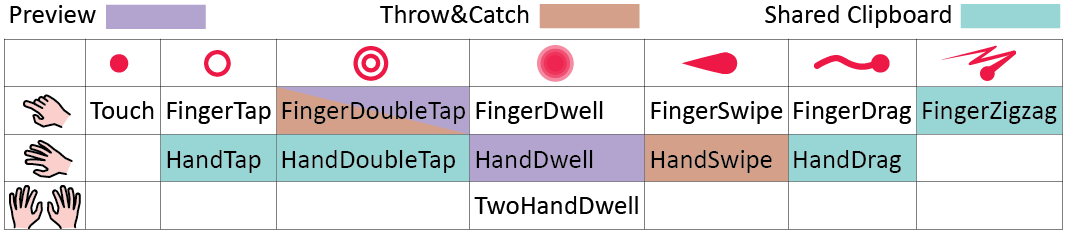
\includegraphics[width=0.5\textwidth]{images/RecognizedGestures.png}
        \caption{Figure 1. image taken from the source article (Fig2)}
        \label{fig:myimage}
    \end{figure}
    
    \indent \indent So these three recognized gestures were implemented in the prototype, and they're meant to facilitate data-centric
    collaborative tasks on large interactive surfaces. Plus these are especially the pattern gestures that can be applied \& used by a couple of users in a 
    tasks. Below are detailled these three different gestures and their uses.

    \begin{itemize}
        \item \textit{Throw and Catch :} \newline 
        \item \textit{Preview :} \newline 
        \item \textit{Shared Clipboard} \newline 
    \end{itemize}

    \paragraph{ \textit{Study 1 :}
                \newline}
    
    \paragraph{ \textit{Study 2 :}
                \newline 
                \indent \indent \textnormal{} }
            
    \paragraph{ \textit{Discussion :}
                \newline
                \indent \indent \textnormal{} }
    
    \paragraph{ \textit{Conclusion :}
                \newline
                \indent \indent \textnormal{} }
    
    \newpage

    \label{sec:liu2014}
    \subsection{Effects of Display Size and Navigation Type on a Classification Task}
    \subparagraph{by : C.Liu, O.Chapuis, M.Beaudouin-Lafon, E.Lecolinet, W.Mackay}
    \cite{liu2014effects}
    \paragraph{ \textit{Quick Summary :} 
                \newline
                \indent \indent \textnormal{} }
    
    \paragraph{ \textit{Experiment Idea :} 
                \newline
                \indent \indent \textnormal{} }

    \paragraph{ \textit{First Experiment :} 
                \newline
                \indent \indent \textnormal{} }

    \paragraph{ \textit{Second Experiment :} 
                \newline
                \indent \indent \textnormal{} }

    \paragraph{ \textit{Discussion :}
                \newline
                \indent \indent \textnormal{} }
                
    \paragraph{ \textit{Conclusion :}
                \newline
                \indent \indent \textnormal{} }

    \label{sec:liu2016}
    \subsection*{Shared Interaction on a Wall-Sized Display in a Data Manipulation Task}
    \subparagraph{by : C.Liu, O.Chapuis, M.Beaudouin-Lafon, E.Lecolinet, W.Mackay}
    \cite{liu2016shared}

    \begin{multicols}{2}
        \paragraph{ \textit{Quick Summary :} 
                \newline }
        \indent \indent As wall-sized displays are now becoming one of the most used technologies when it comes to data manipulations, knowing the benefits and drawbacks of using LHRD seems as interesting as important. And so this article does 
        it by comparing these to their desktop monitors  equivalents, for a task that involves explicit data manipulation. The purpose of the article is to conduct a controlled experiment to compare the performance of physical navigation in 
        front of a wall-size display with virtual navigation using pan-and-zoom on a desktop monitor for this task. The authors aim to understand the interaction effect between display type and task difficulty and to develop guidelines 
        for designing displays for interactive tasks that involve data manipulation. Overall, the article seeks to contribute to a deeper understanding of the advantages and drawbacks of wall-size displays compared to desktop monitors and to 
        provide insights for the design of displays for complex tasks.

        \paragraph{ \textit{Experiment Idea :} 
                \newline }
        \indent \indent The conducted experiment was an abstract classification task where users had to divide \& sort items into classes depending on their properties. Searchers used a middle ground approach where there were more containers than classes, 
        and then users would have to place those items into containers without letting the container overflow. The task required users to determine when two items were in the same class, which was represented by a different letter. Information density was 
        operationalized by adjusting font size. The experimenters controlled the complexity of the task through several parameters, including the number of items, classes, containers, and label font size. This approach provides a rich yet easy-to-control 
        design space for experimental tasks based on the abstract task. The experimenters compared the benefits and drawbacks of wall-sized displays and desktop displays in this classification task.

        \paragraph{ \textit{First Experiment :} 
                \newline }
        \indent \indent This first experiment compared user's performance, subjective experiences, and preferences when distinctly using a desktop computer and a large wall display for a pick-and-place task. The experiment used three different label sizes 
        and two levels of task difficulty. The results show that participants' performances were significantly better on the wall display than on the desktop, especially for the harder task and the medium label size. The wall display also resulted in lower 
        subjective mental load and frustration. Almost all participants preferred the wall display, except for the large label size. The study found a strong interaction effect between the display type and the label size, where the desktop with large labels 
        was fast but exploring small and medium labels was painful. Participants also reported different senses of engagement between the desktop and the wall display, where the desktop gave a sense of control while the wall display gave a sense of being part 
        of the interaction.

        \paragraph{ \textit{Second Experiment :} 
                \newline }
        \indent \indent This second experiment aims to test whether virtual navigation techniques on a desktop interface can beat physical navigation on a wall-size display for difficult classification tasks. In this one, researchers compared three different desktop 
        techniques for difficult classification tasks: a baseline pan-and-zoom (PZ) technique, an overview+detail (PZ+OV) technique, and a focus+context (Fisheye) technique. They recruited 12 volunteers aged 22 to 38 with normal or corrected vision and used a within-subjects design. 
        The results showed no significant difference in task completion time between the three techniques, and none of the techniques were as effective as physical navigation on a wall-size display for this task. Nine participants preferred the Fisheye technique, while three preferred PZ+OV.*
        But still, it  showed that physical navigation on a wall-size display outperformed virtual navigation using desktop techniques for difficult classification tasks. Despite the fact that the focus+context and overview+detail desktop techniques performed similarly to the pan-and-zoom 
        technique in terms of task completion time, none of them came close to the performance of physical navigation on the wall-size display. Additionally, while the fisheye lens technique was preferred by some participants, others found it difficult to control and focus on labels despite its 
        high magnification factor. Overall, the experiment confirmed the superiority of physical navigation on a wall-size display for complex data manipulation tasks compared to desktop techniques.

        \paragraph{ \textit{Discussion :}
                \newline }
        \indent \indent In the \textit{CONCLUSION AND FUTURE WORK} part, the statement is that a wall-size display can be more efficient than a desktop display for difficult data classification tasks that involve data manipulation, especially when there is a high information density. 
        Moreover, thanks to the experiment that compared physical navigation in front of a wall-size display with virtual navigation on a desktop display. Authors found that the desktop display was more efficient for easy tasks, but the wall-size display was significantly more efficient 
        (up to 35\%) for difficult tasks. They suggest that this is just the first step in understanding the benefits of wall-size displays and that future research should investigate collaborative work and new techniques for improving user performance and reducing cognitive load in 
        both wall and desktop environments.

        \paragraph{ \textit{Conclusion :}
                \newline }
        \indent \indent My personal conclusion would be that the choice of display size and navigation technique can significantly impact user performance for certain types of tasks. This may have implications for the design of user interfaces and visualizations, especially for complex 
        data manipulation tasks. The study highlights the need for further research to understand the interaction environment provided by wall-size displays, particularly in collaborative work settings. Additionally, the study suggests that a deeper understanding of spatial memory and 
        the respective advantages of physical and virtual navigation could inform the design of new techniques for both wall and desktop environments to improve user performance and reduce cognitive load.
    \end{multicols}
    
\end{document}